\documentclass[a4paper,12pt]{article} % Tipo de documento y tamaño de letra.
\usepackage[utf8]{inputenc} % Para que reconozca caracteres especiales como tildes.
\usepackage[spanish]{babel} % Para definir el idioma y el formato de fechas en español.
\usepackage{amsmath, amssymb} % Paquetes para símbolos y ecuaciones avanzadas (Para hacer una ecuación con un recuadro).
\usepackage{ragged2e} % Para justificar textos.
\usepackage{multicol} % Para crear columnas.
\usepackage{slashed} % Para generar números o variables canceladas (Una línea diagonal sobre el número o variable).
\usepackage{graphicx} % Paquete para poner graficas.
\usepackage{float} % Para poder dejar la imagen en un punto fijo del documento.
\usepackage{longtable} % Para tablas largas.
\usepackage{cancel} % Para hacer cancelaciones en medio de operaciones.
\usepackage{xcolor} % Para el color y esas cosas.
\usepackage{apacite} % Paquete para citas APA.
\usepackage{fancyhdr} % Para personalizar encabezados y pies de página.
\usepackage{geometry} % Para ajustar márgenes.
\usepackage{setspace} % Para ajustar el interlineado.
\usepackage{natbib} % Para manejar las citas y que no queden pegadas y feas :P.
\usepackage{hyperref} % Para que los enlaces funcionen con su URL.
\usepackage[version=4]{mhchem}  % Versión recomendada para mayor funcionalidad.
\usepackage{chemfig} %También para hacer estructuras químicas.
\usepackage{array} % Para mejor control de las columnas.
\usepackage{siunitx} % Para unidades físicas.
\usepackage{booktabs}
\usepackage{siunitx}
\usepackage[table]{xcolor} % Para colores
\usepackage{multirow}










\pagestyle{fancy}
\fancyhf{} % Limpia encabezados y pies de página predeterminados
\fancyhead[L]{\textbf{SIMULACIONES QUÍMICAS.}} % Encabezado izquierdo
\fancyhead[R]{\textbf{QUÍMICA.}} % Encabezado derecho
\fancyfoot[C]{\thepage} % Número de página en el centro del pie

\geometry{headheight=12.96115pt, top=1in, bottom=1in, left=1in, right=1in}
\begin{document}

\begin{figure}[H] 
    \centering
    
\includegraphics[width=0.5\textwidth]{Unir.jpg} 
\end{figure}

\vspace{\baselineskip}

% Ajustamos manualmente todo ;)
\begin{center}
    \textbf{\Large } \\[0.3cm]
    \vspace{\baselineskip}
    \textbf{Liz Ángel Núñez Torres} \\[0.4cm]
    \textbf{Grado en Física} \\[0.4cm]
    \textbf{Universidad Internacional de La Rioja} \\[0.4cm]
    \textbf{9 de Junio de 2025}
\end{center}



\newpage

\tableofcontents

\newpage

\section*{Módulos de simulación.}
\addcontentsline{toc}{section}{Introducción}

\vspace{\baselineskip}

\begin{enumerate}
    \item Determinar la cantidad de un reactivo que se encuentra en una muestra, convirtiéndolo
    mediante una reacción química en otro compuesto conocido que puede ser aislado y pesado. 
    Calcula la cantidad de cloro que tiene el cloruro desconocido y razona tu respuesta. 
    ¿Qué sucede con el exceso de \ce{AgNO3} añadido a la disolución?

    \item Determina la constante de la velocidad de reacción, así como los órdenes de reacción
    respecto a cada uno de los compuestos. Debes mostrar los cálculos y las gráficas,
    así como explicar todos los resultados obtenidos 

    \begin{itemize}
        \item Mantener constante la concentración de [\ce{H2O2}] mientras variamos [\ce{I^-}]
        \item Mantener constante [\ce{I^-}] variando la concentración [\ce{H2O2}]. 
    \end{itemize}
\end{enumerate}

\vspace{\baselineskip}

\section{Análisis Gravimétrico de Cloruros.}

\vspace{\baselineskip}

\begin{justify}
\textbf{El procedimiento será.}
\end{justify}

\begin{enumerate}
    \item Obtención de la muestra desconocida.
    \item Añadir agua a la muestra de XCl.
    \item Añadir ácido nítrico concentrado.
    \item Añadir \ce{AgNO3} 1M.
    \item Filtrar y pesar el \ce{AgCl}
\end{enumerate}


\vspace{\baselineskip}

\subsection{Obtención de la muestra desconocida.}


\begin{figure}[H]
    \centering
    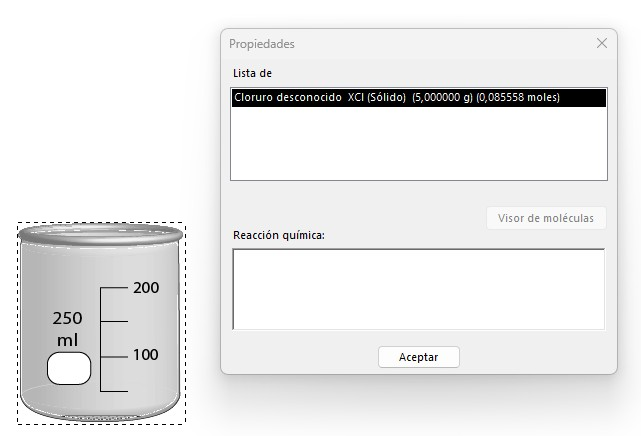
\includegraphics[width=0.7 \textwidth]{Paso1.jpg}
    \caption{Vaso de 250 mL con \(5g\) de clocuro \ce{XCl} desconocido.}
\end{figure}

\vspace{\baselineskip}

\subsection{Añadir agua a la muestra de XCl}

\begin{figure}[H]
    \centering
    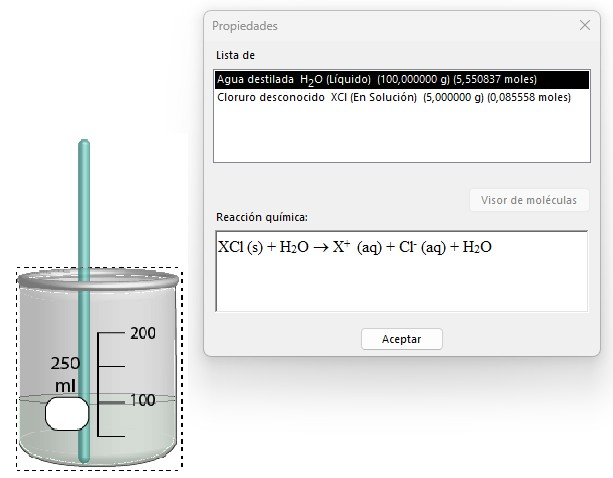
\includegraphics[width=0.7 \textwidth]{paso2.jpg}
    \caption{Vaso con 100 mL de agua siendo agitada hasta la disolución de la muestra.}
\end{figure}

\vspace{\baselineskip}

\subsection{Añadir ácido nítrico concentrado.}

\begin{figure}[H]
    \centering
    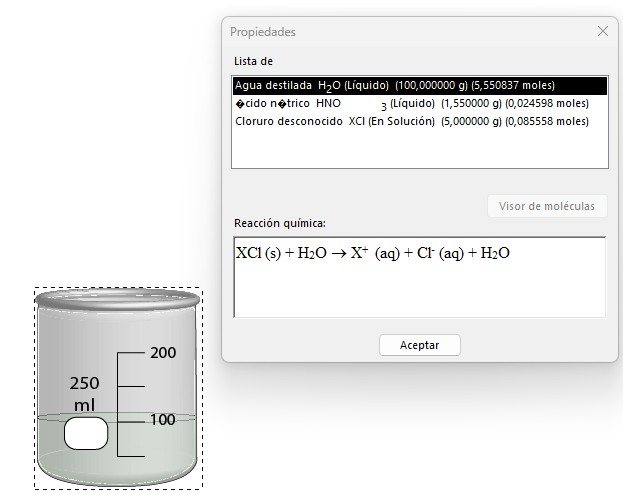
\includegraphics[width=0.7 \textwidth]{paso3.jpg}
    \caption{Vaso con 1 mL de \ce{HNO3} concentrado a la disolución de XCl.}
\end{figure}

\vspace{\baselineskip}

\subsection{Añadir \ce{AgNO3} 1M.}

\begin{figure}[H]
    \centering
    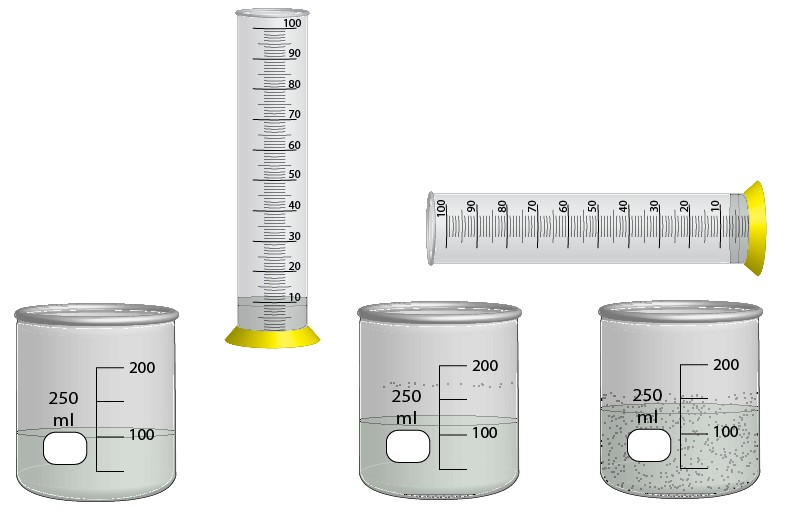
\includegraphics[width=0.7 \textwidth]{paso4.jpg}
    \caption{Con la probeta, en incrementos de 9 dosis de 10 mL de \ce{AgNO3} 1M hasta un total de 90 mL, consumimos el cloruro XCl desconocido (en la imagen se muestra el procedimiento y el precipitado). }
\end{figure}

\vspace{\baselineskip}

\subsection{Filtrar y pesar el \ce{AgCl}.}

\begin{figure}[H]
    \centering
    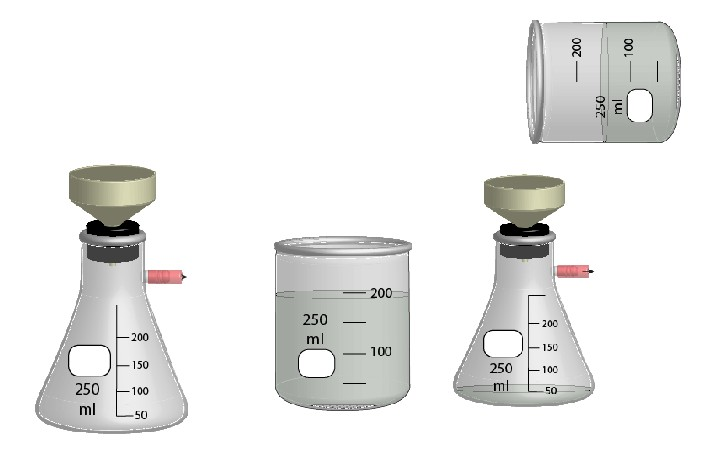
\includegraphics[width=0.7 \textwidth]{paso5.jpg}
    \caption{Usamos el embudo Buchner en un matraz de 250 mL donde verteremos el contenido para filtrar el precipitado.}
\end{figure}


\begin{figure}[H]
    \centering
    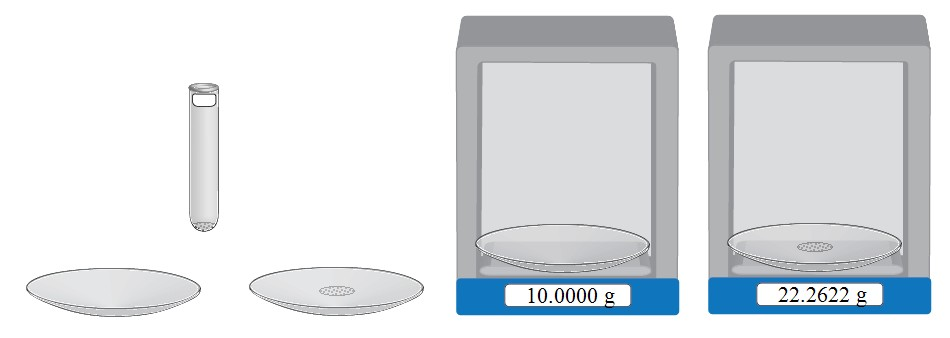
\includegraphics[width=0.7 \textwidth]{paso5.1.jpg}
    \caption{Ponemos el precipitado en un tubo de ensayo de 50 mL. Posteriormente dejaremos el precipitado en un vidrio de reloj para pesar el mismo en una balanza de presición, no sin antes obtener el peso neto del vidrio de reloj donde la diferencia entre su peso y el peso con el precipitado nos arroja la masa de \ce{AgCl}.     }
\end{figure}

\vspace{\baselineskip}

\subsection{Observaciones.}


\begin{table}[H]
\centering
\renewcommand{\arraystretch}{1.2} % Espaciado vertical
\begin{tabular}{| m{12cm} | m{3cm} |} % Columnas: negrita en la primera, justificada en la segunda
\hline
Masa de la muestra desconocida (g) &  5g. \\ \hline
Masa del precipitado de AgCl &  12.26g. \\ \hline
Volumen aproximado de disolución de AgNO3 añadido (mL) &  \( \simeq \)  90 mL. \\ \hline
Moles de AgCl &  0.0855 moles.  \\ \hline
Masa de \ce{Cl^-} en la muestra de XCl  & 3.03g. \\ \hline
Porcentaje de \ce{Cl^-} en la muestra desconocida &   60.62\%. \\ \hline
\end{tabular}
\end{table}

\newpage

\begin{justify}
    \textbf{¿Qué sucede con el exceso de \ce{AgNO3} añadido a la disolución?}
\end{justify}

\begin{justify}
    El exceso de \ce{AgNO3} se disuelve en la disolución como iones \ce{Ag^+} y \ce{NO3^-} libres, sin formar más precipitado,
    esto nos confirma que se ha efectuado toda la reacción del \ce{Cl^-} de la muestra desconocida \ce{XCl}.
\end{justify}


\vspace{\baselineskip}

\section{Cinética de una reacción Redox.}

\begin{justify}
    El procedimiento \textbf{general} será (Procederemos varias veces en cada punto).
\end{justify}

\begin{enumerate}
    \item Preparar una disolución de tiosulfato sódico.
    \item Preparar la disolución de yoduro de potasio.
    \item Añadir las disoluciones de \ce{KI} y \ce{Na2S2O3} .
    \item Añadir \ce{H2O2} de 0,1M y contar el tiempo de la reacción.
    \item Variando [H2O2] y manteniendo [I-] constante.  

\end{enumerate}

\begin{justify}
    Donde omitiremos los pasos reiterativos del 1 hasta el 4, siendo los pasos 5 y 6 los únicos que
    detallaremos en cada caso.
\end{justify}


\subsection{Preparación del tiosulfato sódico.}

\begin{figure}[H]
    \centering
    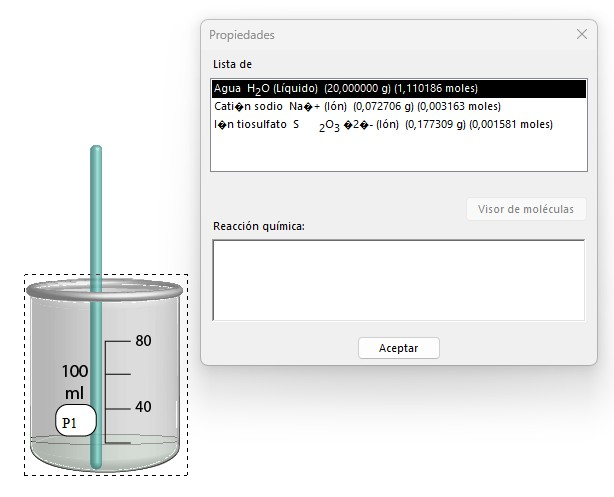
\includegraphics[width=0.7 \textwidth]{paso2.1.jpg}
    \caption{Preparación del \textbf{tiosulfato sódico} con 0.25g de \ce{Na2S2O3} y 20 mL de \ce{H2O}. }
\end{figure}

\vspace{\baselineskip}

\subsection{Preparación del yoduro de potasio.}

\begin{figure}[H]
    \centering
    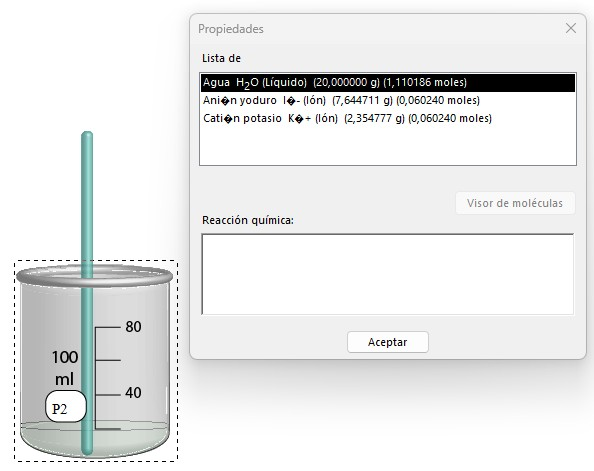
\includegraphics[width=0.7 \textwidth]{paso2.2.jpg}
    \caption{Preparación del \textbf{yoduro de potasio} con 10g \ce{Kl} y 20 mL de \ce{H2O}. }
\end{figure}


\vspace{\baselineskip}

\subsection{Añadir las disoluciones.}

\begin{figure}[H]
    \centering
    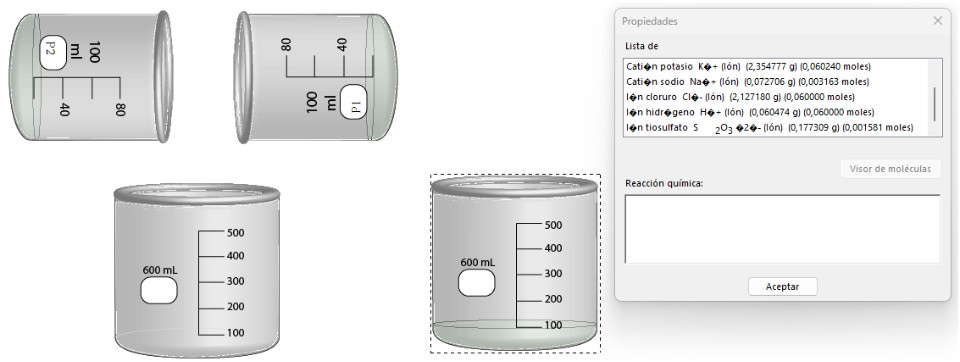
\includegraphics[width=0.9 \textwidth]{paso2.3.jpg}
    \caption{En un vaso de 600 mL añadimos las disoluciones de \ce{Kl} y \ce{Na2S2O3} y posteriormente 60 mL de \ce{HCl} 1M. }
\end{figure}

\subsection{Añadir perióxido de hidrógeno \ce{H2O2}.}

\begin{figure}[H]
    \centering
    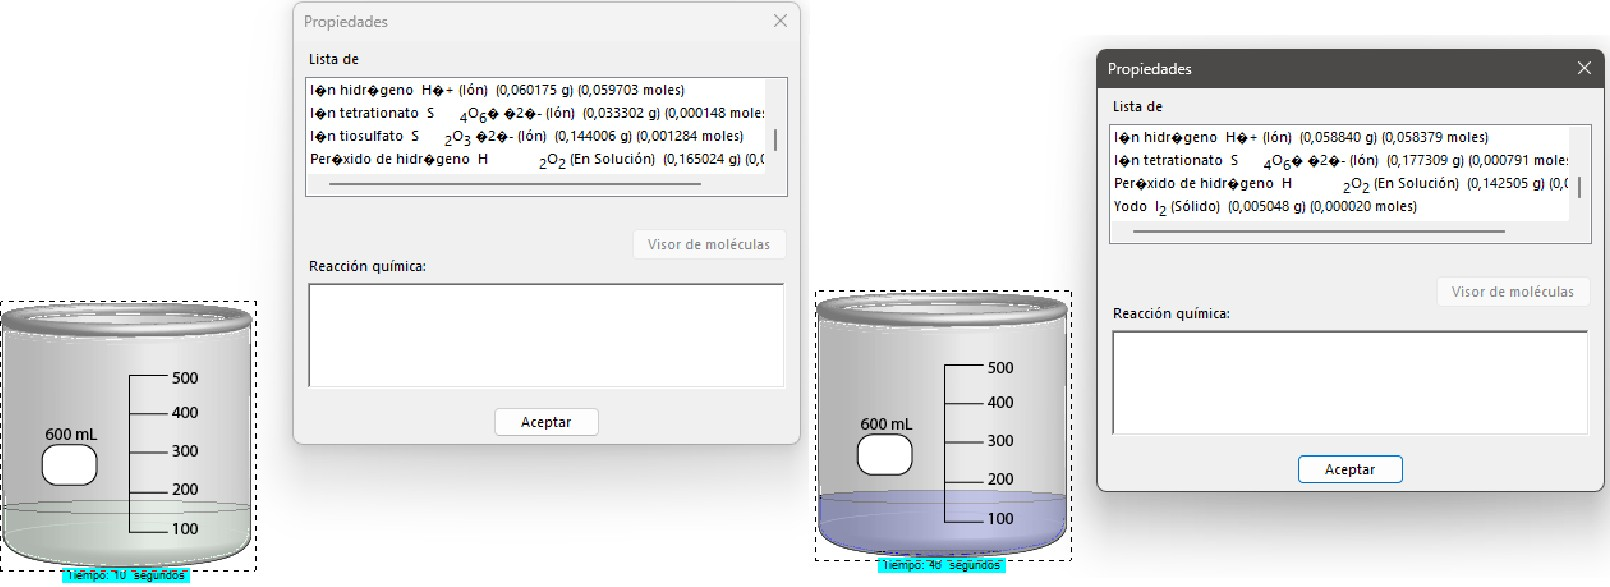
\includegraphics[width=0.9 \textwidth]{paso2.4.jpg}
    \caption{Vaso al agregar 50 mL de \ce{H2O2} e iniciar y  terminar la reacción al manifestarse el yodo.}
\end{figure}


\vspace{\baselineskip}

\subsection{Variación de \ce{[H2O2]} y \ce{[I^-]} constante. }

\begin{figure}[H]
    \centering
    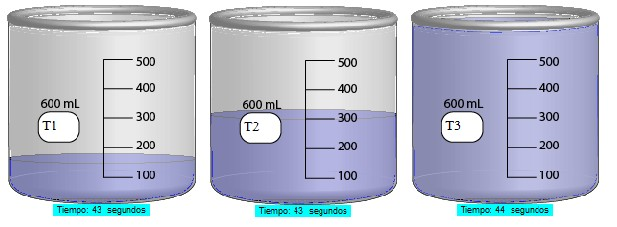
\includegraphics[width=0.8 \textwidth]{paso2.5.jpg}
    \caption{\textbf{Vaso T1}, con \ce{Kl} = 10g, tiempo de reacción 43s.}
    \caption{\textbf{Vaso T2}, con \ce{Kl} = 20g, 150 mL de excedente en \ce{H2O}, tiempo de reacción 43s.}
    \caption{\textbf{Vaso T2}, con \ce{Kl} = 40g, 450 mL de excedente en \ce{H2O}, tiempo de reacción 44s.}
\end{figure}

\vspace{\baselineskip}

\subsection{Variación de  \ce{[I^-]} y \ce{[H2O2]} constante. }


\begin{figure}[H]
    \centering
    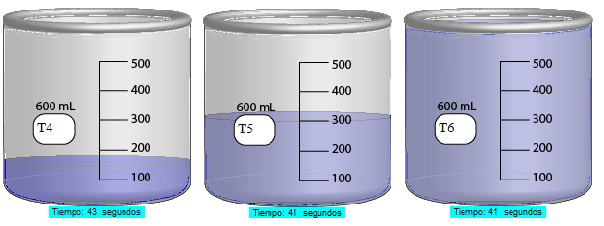
\includegraphics[width=0.8 \textwidth]{paso2.6.jpg}
    \caption{\textbf{Vaso T4}, con \ce{H2O2} = 50 mL, tiempo de reacción 43s.}
    \caption{\textbf{Vaso T5}, con \ce{H2O2} = 100 mL, 100 mL de excedente en \ce{H2O}, tiempo de reacción 41s.}
    \caption{\textbf{Vaso T6}, con \ce{H2O2} = 200 mL, 200 mL de excedente en \ce{H2O}, tiempo de reacción 41s.}
\end{figure}

\vspace{\baselineskip}

\subsection{Observaciones. }

\begin{table}[H]
\centering
\footnotesize
\begin{tabular}{||c|c|c|c|c|c|c|c||}
\toprule
Reacción. & $[\text{H}_2\text{O}_2]$ & $[\text{I}^-]$ & Tiempo & Velocidad & $\log[\text{H}_2\text{O}_2]$ & $\log[\text{I}^-]$ & $\log(v)$ \\
& (\si{M}) & (\si{M}) & (\si{s}) & (\si{M.s^{-1}}) & & & \\
\midrule
1 & 0.033 & 0.402 & 43 & 1.22e-4 & -1.48 & -0.40 & -3.91 \\
2 & 0.017 & 0.402 & 43 & 6.12e-5 & -1.78 & -0.40 & -4.21 \\
3 & 0.008 & 0.402 & 44 & 2.99e-6 & -2.08 & -0.40 & -5.52 \\
4 & 0.033 & 0.402 & 43 & 1.22e-4 & -1.48 & -0.40 & -3.91 \\
5 & 0.033 & 0.201 & 41 & 6.42e-5 & -1.48 & -0.70 & -4.19 \\
6 & 0.033 & 0.100 & 41 & 3.21e-5 & -1.48 & -1.00 & -4.49 \\
\bottomrule
\end{tabular}
\caption{Tabla de valores respecto a las reacciones.}
\end{table}

\subsection{Gráfica y constante de velocidad K.}

\begin{figure}[H]
    \centering
    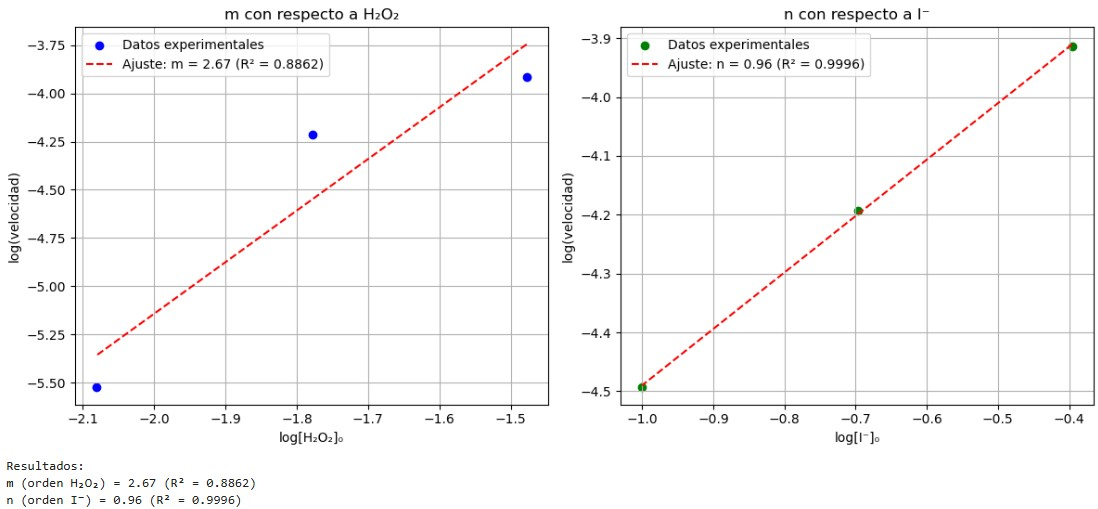
\includegraphics[width=1.0 \textwidth]{Pasf..jpg}
    \caption{Gráficas de n y m.}
\end{figure}



\begin{justify}
    Considerando los órdenes de reacción determinados experimentalmente:
\end{justify}

\[
\boxed{v = k \cdot [\text{H}_2\text{O}_2]^{2.67} \cdot [\text{I}^-]^{0.96}}
\]

Donde:
\begin{itemize}
    \item $v$ es la velocidad de reacción en \si{M.s^{-1}}
    \item $k$ es la constante de velocidad
    \item Los exponentes son los órdenes parciales determinados gráficamente
\end{itemize}


\section*{Cálculo de la Constante de Velocidad ($k$)}

\begin{enumerate}
\item \begin{justify}
    Usando los datos de la \textbf{Reacción 1}:
\end{justify}

\[v = 1.22 \times ^{-4} Ms^{-1}\]

\[[\ce{H2O2}] = 0.0333 M\]

\[[\ce{I^-}] = 0.402 M \]

\item \textbf{Despeje de $k$} (asumiendo $m = n = 1$):
\[
k = \frac{v}{[\text{H}_2\text{O}_2] \cdot [\text{I}^-]} = \frac{1.22 \times 10^{-4}}{0.0333 \times 0.402}
\]

\item \textbf{Resultado}:
\[
\textcolor{blue}{\boxed{k = 9,2 \times 10^{-3} \; L/mol \cdot s }}
\]
\end{enumerate}


\section{Calificación/Observaciones.}

\begin{figure}[H]
    \centering
    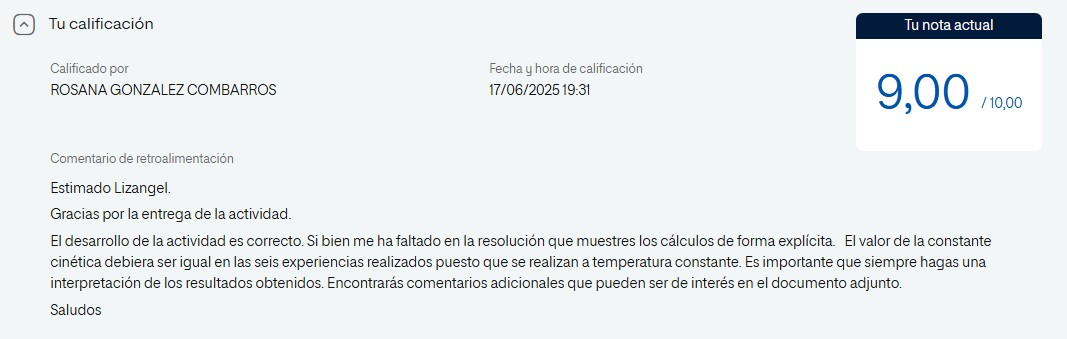
\includegraphics[width=1 \textwidth]{calificacion.jpg}
\end{figure}





\end{document}